\part{Introduction}
\frame{\partpage}

\begin{frame}
	\begin{itemize}
		\pause \item When we start the optimisation process in games, we want to check if we are CPU or GPU bound
		\pause \item Once this is identified then we can start looking at different ways of optimising our code
		\begin{itemize}
			\pause \item System Level
			\pause \item Algorithm
			\pause \item Micro 
		\end{itemize}
		\pause \item In this session we are going to assume our application is CPU bound 
	\end{itemize}
\end{frame}

\begin{frame}{Optimisation Flow}
	\begin{figure}
		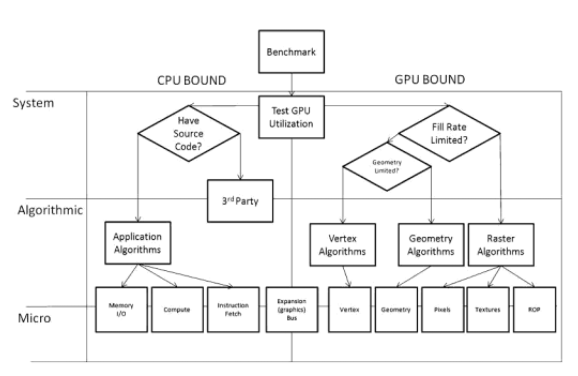
\includegraphics[width=1.0\textwidth,height=0.8\textheight]{OptimisationFlowChart}  
	\end{figure}
\end{frame}